% =======================================================================================
\section{The LISA Galactic-Binary Problem}
\label{sec:gw}
% =======================================================================================

We address the \acp{gb} of the \ac{lisa} data alone, in stationary noise of known spectrum, a first
step towards an amortised global fit (\cref{sec:followups}).

\subsection{Signal, Noise and Prior}
\label{sec:gw-data}\label{sec:gw-waveforms}\label{sec:gw-priors}

A \ac{gb} is a circular, slowly chirping binary of white dwarfs that emits a quasi-monochromatic
\ac{gw} at twice its orbital frequency \citep{nelemans2001gravitational,korol2017prospects}. Eight
parameters describe it,
\begin{equation}
  \theta = (f_0,\fdot,\Amp,\alpha,\delta,\psi,\iota,\phi_0):
  \label{eq:gw-parameters}
\end{equation}
frequency and frequency derivative at the start of the observation, strain amplitude, right
ascension and declination, polarisation angle, inclination and initial phase. Over the observation
time $\Tobs=\qty{\ForwardModelTobsYears}{\year}$ the detector's orbit modulates the signal, which
locates the source on the sky and spreads it over neighbouring frequency bins of width $1/\Tobs$.
JaxGB \citep{jaxgb} simulates the response in the noise-orthogonal \ac{tdi} channels $A$, $E$, $T$
\citep{tinto2021time,prince2002lisa} on the \ac{gpu}, so every training window is simulated on the
fly (\cref{app:forward-model}).

The noise is the stationary Gaussian instrument noise of the \ac{lisa} requirements
\citep{lisasst2018lisa,babak2021lisa}, with one-sided \ac{psd} $S_c(f)$ in channel $c$
(\cref{app:noise}). On the Fourier bins $f_k = k/\Tobs$, with $\tilde h_c(f;\theta_s)$ the response of
source $s$, the data of a band holding $N$ sources are
\begin{equation}
\begin{aligned}
  \tilde d_{k,c} &= \sum_{s=1}^{N}\tilde h_c(f_k;\theta_s) + \tilde n_{k,c},\\
  \tilde n_{k,c} &\sim \CN\!\bigl(0,\ P_c(f_k)\bigr),\qquad
  P_c(f) = \tfrac12\,S_c(f)\,\Tobs,
\end{aligned}
  \label{eq:noise-data}
\end{equation}
independent across bins and channels. A source's \ac{snr} is that of its response alone
\citep{cutler1994gravitational},
\begin{equation}
  \snr_s^2 = 4\sum_{c}\sum_{k}\frac{\bigl|\tilde h_c(f_k;\theta_s)\bigr|^2}{S_c(f_k)\,\Tobs},
  \label{eq:gw-snr}
\end{equation}
and we call a source \emph{visible} when $\snr\ge\RatesVisibleSnr$. The \ac{snr} accumulates over the
many bins a response spans, so per bin even a visible source stands little above the noise
(\cref{fig:forward-model-window}).

\begin{figure}[t]
  \centering
  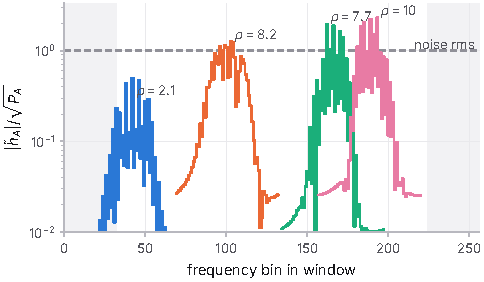
\includegraphics[width=\columnwidth]{figures/training-window.pdf}
  \caption{Visible sources stand little above the noise per bin. The \acs{tdi}-1.5 response in channel $A$
  of each \ac{gb} of one narrow-band window, in units of the noise's root-mean-square per bin, labelled
  with its \acs{snr}.}
  \label{fig:forward-model-window}
\end{figure}

The $S_w$ sources of a window $w$ centred on $\fw$, $\Theta_w = (\theta_1,\dots,\theta_{S_w})$, are
independent draws from one per-source prior $\pi_w(\theta) = \pi(\theta\mid\fw)$,
\begin{equation}
  \pi_w(\Theta_w) = \prod_{s=1}^{S_w}\pi_w(\theta_s),
  \label{eq:priors-window-prior}
\end{equation}
fitted to a simulated Galactic catalogue of double white dwarfs
\citep{perego2025towards,breivik2020cosmic} (\cref{tab:priors-source}, \cref{fig:priors},
\cref{app:priors-sources}). It is closer to a real population than the flat or log-flat priors of
other analyses \citep{strub2022bayesian,deng2025modular,delmond2026neural}, and it is broad: most of
its sources lie below the noise.

\begin{table}[t]
\caption{The prior of one source in window $w$: a Gaussian in the logarithms of $(f_0,\fdot,\Amp)$,
with $f_0$ truncated to the window, a catalogue sky and an isotropic orientation.}
\label{tab:priors-source}
\centering
\footnotesize
\begin{tabular}{@{}lp{0.68\columnwidth}@{}}
\toprule
parameter & prior \\
\midrule
$(f_0, \fdot, \Amp)$ & $(\log_{10}f_0, \log_{10}\fdot, \log_{10}\Amp)\sim\Normal(\mu_\pi, \Sigma_\pi)$, \cref{eq:priors-source} \\
$(\alpha, \delta)$ & bulge + disc, \cref{eq:priors-sky} \\
$\psi$ & $\Unif(0, 2\pi)$ \\
$\iota\in[0,\pi]$ & $\cos\iota\sim\Unif(-1, 1)$ \\
$\phi_0$ & $\Unif(0, 2\pi)$ \\
\bottomrule
\end{tabular}
\end{table}

\begin{figure*}[t]
  \centering
  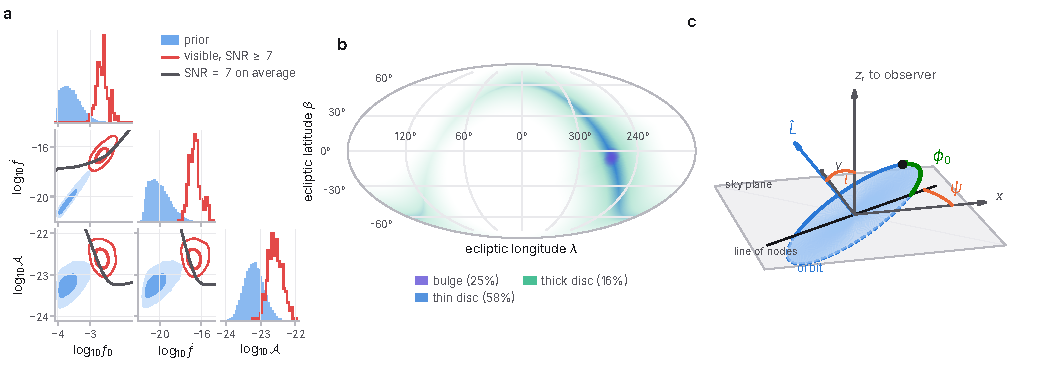
\includegraphics[width=\textwidth]{figures/priors.pdf}
  \caption{The per-source prior is broad and mostly below the noise. (a)~$(\log_{10}f_0, \log_{10}\fdot, \log_{10}\Amp)$ over the full band,
  \num{\ChartPriorDraws} sources in windows centred on the catalogue's $f_0$ marginal: regions
  enclosing \qty{\PriorCornerInner}{\percent} and \qty{\PriorCornerOuter}{\percent} of the prior
  (blue) and of the sources with $\snr\ge\PriorsVisibleSnr$ (red), and the line
  $\snr=\PriorsVisibleSnr$ (grey), which averages over the other parameters, so sources
  that reach it through a favourable sky or orientation also lie below it. (b)~The sky,
  \cref{eq:priors-sky}, in ecliptic coordinates $(\lambda, \beta)$: the bulge, the thick and the thin
  disc, each shaded over three decades of its density. (c)~The orientation: the orbit (blue, dashed
  below the sky plane) is inclined by $\iota$ to the sky plane $(x, y)$; its line of nodes is at
  $\psi$ from $x$, and $\phi_0$ is the phase along the orbit at the start of the observation.}
  \label{fig:priors}
\end{figure*}

\subsection{Likelihood and Windows}
\label{sec:gw-slicing}\label{sec:gw-factorisation}\label{sec:gw-windows}

The noise is stationary, so the likelihood is diagonal in frequency, and a \ac{gb}'s response covers
only $R$ bins around $f_0\Tobs$ (\cref{sec:narrow-band}), so each bin involves only the sources whose
responses reach it. We therefore cut the band into windows of $K = \ForwardModelWindowResponses{}R$
bins. A source belongs to the window whose interior holds its $f_0$, and a guard band of $R/2$ bins
at each edge keeps its whole response inside (\cref{app:forward-model-windows}). With $d_w$ the data
of window $w$, the posterior of all the band's sources $\Theta$ factorises,
\begin{equation}
\begin{gathered}
  p(\Theta\mid d) = \textstyle\prod_{w} p(\Theta_w\mid d_w),\\
  p(\Theta_w\mid d_w) \propto p(d_w\mid\Theta_w)\,\pi_w(\Theta_w),
\end{gathered}
  \label{eq:gw-factorisation}
\end{equation}
with the Whittle likelihood
\begin{equation}
  \log p(d_w\mid\Theta_w) = -\sum_{k\in w}\sum_{c}\frac{\bigl|\tilde d_{k,c}-\sum_{s\in w}\tilde h_c(f_k;\theta_s)\bigr|^2}{P_c(f_k)}
  \label{eq:loglik}
\end{equation}
up to a constant. One network conditioned on $\fw$ then serves the whole band, window by window and in
parallel. It reads the window whitened, $y\in\R^{K\times6}$, the real and imaginary parts of
$\tilde d_{k,c}$ in the three channels divided by $\sqrt{P_c(f_k)/2}$, and its target is
$p(\Theta_w\mid y,\fw) = p(\Theta_w\mid d_w)$. In real data the wings of loud neighbours break the
factorisation, and a global fit updates overlapping segments in turn \citep{littenberg2020global}
(\cref{sec:followups}).
